% Created 2016-06-26 Sun 00:29
\documentclass[11pt]{article}
\usepackage[utf8]{inputenc}
\usepackage[T1]{fontenc}
\usepackage{fixltx2e}
\usepackage{graphicx}
\usepackage{longtable}
\usepackage{float}
\usepackage{wrapfig}
\usepackage{rotating}
\usepackage[normalem]{ulem}
\usepackage{amsmath}
\usepackage{textcomp}
\usepackage{marvosym}
\usepackage{wasysym}
\usepackage{amssymb}
\usepackage{capt-of}
\usepackage[hidelinks]{hyperref}
\tolerance=1000
\usepackage[utf8]{inputenc}
\usepackage{commath}
\usepackage{pgf}
\usepackage{tikz}
\usetikzlibrary{shapes, arrows}
\usepackage{marginnote}
\usepackage{listings}
\usepackage{enumerate}
\usepackage{algpseudocode}
\usepackage{algorithm}
\usepackage{mathtools}
\setlength{\parskip}{16pt plus 2pt minus 2pt}
\renewcommand{\arraystretch}{1.6}
\author{Oleg Sivokon}
\date{\textit{<2016-06-25 Sat>}}
\title{Assignment 18, Data-Structures}
\hypersetup{
  pdfkeywords={Data-Structures, Algorithms, Assignment},
  pdfsubject={Third assignment in the course Data-Structures},
  pdfcreator={Emacs 25.1.50.2 (Org mode 8.2.10)}}
\begin{document}

\maketitle
\tableofcontents


\definecolor{codebg}{rgb}{0.96,0.99,0.8}
\definecolor{codestr}{rgb}{0.46,0.09,0.2}
\lstset{%
  backgroundcolor=\color{codebg},
  basicstyle=\ttfamily\scriptsize,
  breakatwhitespace=false,
  breaklines=false,
  captionpos=b,
  framexleftmargin=10pt,
  xleftmargin=10pt,
  framerule=0pt,
  frame=tb,
  keepspaces=true,
  keywordstyle=\color{blue},
  showspaces=false,
  showstringspaces=false,
  showtabs=false,
  stringstyle=\color{codestr},
  tabsize=2
}
\lstnewenvironment{maxima}{%
  \lstset{%
    backgroundcolor=\color{codebg},
    escapeinside={(*@}{@*)},
    aboveskip=20pt,
    captionpos=b,
    label=,
    caption=,
    showstringspaces=false,
    frame=single,
    framerule=0pt,
    basicstyle=\ttfamily\scriptsize,
    columns=fixed}}{}
}
\makeatletter
\newcommand{\verbatimfont}[1]{\renewcommand{\verbatim@font}{\ttfamily#1}}
\makeatother
\verbatimfont{\small}%
\clearpage

\section{Problem Description}
\label{sec-1}
Implement a program to manage university library.  Below are the operations
the program must support.  The program should use query language given by ABNF
grammar associated to each operation:
\begin{enumerate}
\item \texttt{join\_library(patron, patron\_id)}.
\begin{verbatim}
`+` patron patron_id
\end{verbatim}
Adds a new patron to the library.
\item \texttt{leave\_library(patron, patron\_id)}.
\begin{verbatim}
`-` patron patron_id
\end{verbatim}
Removes existing patron from the library.
\item \texttt{borrow\_book(patron, patron\_id, book\_id)}.
\begin{verbatim}
patron patron_id book_id `+`
\end{verbatim}
Associates given book to patron.
\item \texttt{return\_book(patron, patron\_id, book\_id)}.
\begin{verbatim}
patron patron_id book_id `-`
\end{verbatim}
Dissasocitates the given book and patron.
\item \texttt{list\_books(patron\_id)}.
\begin{verbatim}
`?` patron_id
\end{verbatim}
List all books borrowed by indicated patron.
\item \texttt{who\_borrows(book\_id)}.
\begin{verbatim}
`?` book_id
\end{verbatim}
Displays the patron(s) currnetly holding the indicated book.
\item \texttt{borrows\_most()}.
\begin{verbatim}
`?` `!`
\end{verbatim}
Displays the patron who currently borrows most books.
\end{enumerate}

\section{Discussion}
\label{sec-2}

\subsection{Reflection on assignment}
\label{sec-2-1}
There are several problems with this specification:
\begin{enumerate}
\item It isn't stated whether the same patron can join the library multiple
times, but I assumed patrons may only join the library once.
\item It isn't stated whether it is possible to leave the library while
borrowing any books.  I will treat this as impossible, and will prompt the
user to first return the books to the library.
\item It isn't clear whether leaving multiple times should result in an error.
I will not treat this as an error.
\item It is not clear whether \texttt{book\_id} is akin to ISBN (in which case multiple
copies of the same book may exist), or that \texttt{book\_id} is some internal
library code uniquely marking the book.  I will not treat is as unique.
\item By the same token, it may be possible to return the same book multiple
times, viz when the same patron holds multiple copies of the same book.
\item Consequently, \texttt{who\_borrows} may return the list of patrons (all of which
hold the same book, just not the same exact copy).
\item Some queries provide excess information.  I am going to make the format
more flexible to allow shorter input while preserving the original syntax.
\end{enumerate}

\subsection{Data-structures used to support queries}
\label{sec-2-2}
If it wasn't for \texttt{borrows\_most()}, two \texttt{hash-tables} would fit the bill
perfectly: \texttt{library\_books} table would use book identifiers as keys and
patrons holding these books as values.  Second table, \texttt{library\_patrons} would
use patron identifiers as keys and books held by patrons as values.  Thus,
adding patron to the library would take constant time, removing patron from
the library would also take constant time.  Removing a book from the library
would take constant time (since we can look up \texttt{library\_books} and
immediately discover whether it is held by anyone.  Similarly, \texttt{who\_borrows}
and \texttt{list\_books} would all run in constant time.

The problematic \texttt{borrows\_most} would run in linear time (we would need to
look at all keys in \texttt{library\_patrons} table to find the patron who holds most
books.

We can mitigate this by adding a special slot in the library for the patron
currently holding most books, and then updating this slot any time the
library is modified: for an additional constant memory cost and constant cost
incured on every destructive operation we would perform every operation in
constant time.

\subsection{Extension to queries}
\label{sec-2-3}
To make working with the program more convenient, I will add the following
queries:
\begin{enumerate}
\item \texttt{add\_book}.
\begin{verbatim}
`.` book_id+ `+` | `.` file | `.` num
\end{verbatim}
Adds book to the library.  Book identifier may be repeated several times,
or red from a file or generated by the program.
\item \texttt{show\_library}.
\begin{verbatim}
`?` `?`
\end{verbatim}
This prints the current state of the library, both the books and the
patrons.
\item \texttt{borrow\_book} and \texttt{return\_book} don't need the name of patron returning or
borrowing the book (identifier is enough).  So the patron's name is
optional in the queries.
\end{enumerate}

\section{Solution}
\label{sec-3}
Below is the \texttt{yacc} code for the queries grammar (auxilary code was removed
for brevity).

The parser:
\begin{verbatim}
books   :       BOOKID { $$ = cons($1, NULL); }
        |       BOOKID books { $$ = cons($1, $2); }
        ;

rquery  :       PATRON PATRONID BOOKID PLUS {
                    $$ = query(BORROW, $1, $2, $3); }
        |       PATRON PATRONID BOOKID MINUS {
                    $$ = query(RETURN, $1, $2, $3); }
        |       PLUS PATRON PATRONID {
                    $$ = query(JOIN, $2, $3, NULL); }
        |       MINUS PATRON PATRONID {
                    $$ = query(LEAVE, $2, $3, NULL); }
        |       QUESTION PATRONID {
                    $$ = query(BOOKS, NULL, $2, NULL); }
        |       QUESTION BOOKID {
                    $$ = query(WHO_BORROWS, NULL, NULL, $2); }
        |       QUESTION BANG {
                    $$ = query(BORROWS_MOST, NULL, NULL, NULL); }
        |       QUESTION QUESTION {
                    $$ = query(SHOW, NULL, NULL, NULL); }
        ;

populate :      DOT books { populate_library_list($2); }
        |       DOT QUOTED { populate_library_file($2); }
        |       DOT NUM { populate_library($2); }
        ;

pquery  :       rquery { process_query($1); }
        |       populate {;}
        ;

pqueries :      pquery {;}
        |       pquery pqueries {;}
        ;
\end{verbatim}

And the lexer:
\begin{verbatim}
[+]                      { yylval.str = str(yytext); return PLUS; }
[-]                      { yylval.str = str(yytext); return MINUS; }
[?]                      { yylval.str = str(yytext); return QUESTION; }
[!]                      { yylval.str = str(yytext); return BANG; }
\.                       { yylval.str = str(yytext); return DOT; }
[0-9]{9}                 { yylval.str = str(yytext); return PATRONID; }
[a-zA-Z][a-zA-Z][0-9]{4} { yylval.str = str(yytext); return BOOKID; }
[a-zA-Z]{1,32}           { yylval.str = str(yytext); return PATRON; }
[\"][^\"]+[\"]           { yylval.str = quote(yytext); return QUOTED; }
#[0-9]{1,12}             { yylval.num = atoi(yytext + 1); return NUM; }
[ \t\r\n]+               ;
.                        printf("line: %d, Unexpeced character: %s\n",
                                yylineno, yytext);
\end{verbatim}

No new data-structures are required for solving this task.  The UML diagrams
of the objects involved are given below:

The relevant source files are:
\begin{enumerate}
\item \texttt{assignment18.c} - program's entry point.
\item \texttt{query.c} - query interface.
\item \texttt{library.c} - library data-structure.
\item \texttt{query\_grammar.y} - query parser.
\item \texttt{queries.l} - query lexer.
\end{enumerate}

Documentation for this code is automatically extracted from header files by
\texttt{Doxygen} and stored in \url{../doc} directory.

To compile the code install \href{http://scons.org/doc/0.98.4/HTML/scons-user/x166.html}{SCons}, \href{https://geeksww.com/tutorials/miscellaneous/bison_gnu_parser_generator/installation/installing_bison_gnu_parser_generator_ubuntu_linux.php}{GNU Bison (YACC)}, \href{http://flex.sourceforge.net/}{Flex (LEX)}.  If you
aren't interested in generating from YACC and LEX files, this repository
contains already generated C files and headers.

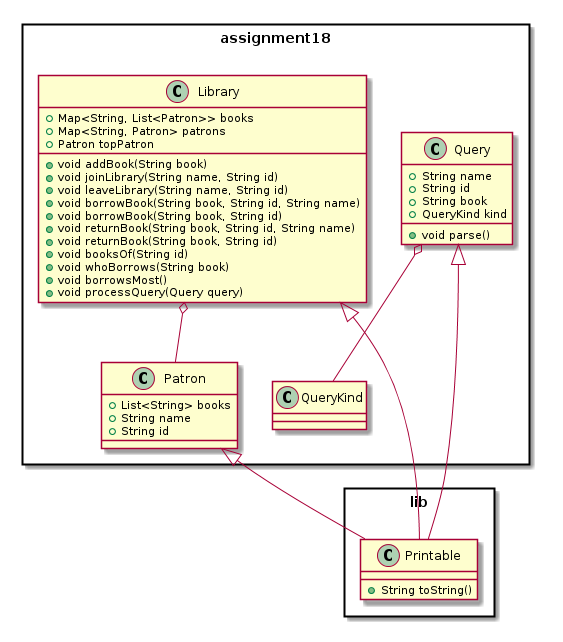
\includegraphics[width=.9\linewidth]{tryout.png}
% Emacs 25.1.50.2 (Org mode 8.2.10)
\end{document}